
%% bare_jrnl.tex
%% V1.4
%% 2012/12/27
%% by Michael Shell
%% see http://www.michaelshell.org/
%% for current contact information.
%%
%% This is a skeleton file demonstrating the use of IEEEtran.cls
%% (requires IEEEtran.cls version 1.8 or later) with an IEEE journal paper.
%%
%% Support sites:
%% http://www.michaelshell.org/tex/ieeetran/
%% http://www.ctan.org/tex-archive/macros/latex/contrib/IEEEtran/
%% and
%% http://www.ieee.org/



% *** Authors should verify (and, if needed, correct) their LaTeX system  ***
% *** with the testflow diagnostic prior to trusting their LaTeX platform ***
% *** with production work. IEEE's font choices can trigger bugs that do  ***
% *** not appear when using other class files.                            ***
% The testflow support page is at:
% http://www.michaelshell.org/tex/testflow/


%%*************************************************************************
%% Legal Notice:
%% This code is offered as-is without any warranty either expressed or
%% implied; without even the implied warranty of MERCHANTABILITY or
%% FITNESS FOR A PARTICULAR PURPOSE! 
%% User assumes all risk.
%% In no event shall IEEE or any contributor to this code be liable for
%% any damages or losses, including, but not limited to, incidental,
%% consequential, or any other damages, resulting from the use or misuse
%% of any information contained here.
%%
%% All comments are the opinions of their respective authors and are not
%% necessarily endorsed by the IEEE.
%%
%% This work is distributed under the LaTeX Project Public License (LPPL)
%% ( http://www.latex-project.org/ ) version 1.3, and may be freely used,
%% distributed and modified. A copy of the LPPL, version 1.3, is included
%% in the base LaTeX documentation of all distributions of LaTeX released
%% 2003/12/01 or later.
%% Retain all contribution notices and credits.
%% ** Modified files should be clearly indicated as such, including  **
%% ** renaming them and changing author support contact information. **
%%
%% File list of work: IEEEtran.cls, IEEEtran_HOWTO.pdf, bare_adv.tex,
%%                    bare_conf.tex, bare_jrnl.tex, bare_jrnl_compsoc.tex,
%%                    bare_jrnl_transmag.tex
%%*************************************************************************

% Note that the a4paper option is mainly intended so that authors in
% countries using A4 can easily print to A4 and see how their papers will
% look in print - the typesetting of the document will not typically be
% affected with changes in paper size (but the bottom and side margins will).
% Use the testflow package mentioned above to verify correct handling of
% both paper sizes by the user's LaTeX system.
%
% Also note that the "draftcls" or "draftclsnofoot", not "draft", option
% should be used if it is desired that the figures are to be displayed in
% draft mode.
%
\documentclass[journal]{IEEEtran}
%
% If IEEEtran.cls has not been installed into the LaTeX system files,
% manually specify the path to it like:
% \documentclass[journal]{../sty/IEEEtran}





% Some very useful LaTeX packages include:
% (uncomment the ones you want to load)


% *** MISC UTILITY PACKAGES ***
%
%\usepackage{ifpdf}
% Heiko Oberdiek's ifpdf.sty is very useful if you need conditional
% compilation based on whether the output is pdf or dvi.
% usage:
% \ifpdf
%   % pdf code
% \else
%   % dvi code
% \fi
% The latest version of ifpdf.sty can be obtained from:
% http://www.ctan.org/tex-archive/macros/latex/contrib/oberdiek/
% Also, note that IEEEtran.cls V1.7 and later provides a builtin
% \ifCLASSINFOpdf conditional that works the same way.
% When switching from latex to pdflatex and vice-versa, the compiler may
% have to be run twice to clear warning/error messages.



\usepackage{pdflscape}
\usepackage{amsfonts}
\usepackage{amsmath}
\usepackage{tikz}
\usetikzlibrary{arrows,positioning}
\usepackage{rotating}
\usepackage{booktabs}

% Custom Macros
\newcommand{\figref}[1]{{Figure}~\ref{#1}}
\newcommand{\tabref}[1]{{Table}~\ref{#1}}
\newcommand{\secref}[1]{{Section}~\ref{#1}}
\newcommand{\appref}[1]{{Appendix}~\ref{#1}}

\hyphenation{MIRACL}

\newcommand{\K}{\ensuremath{\mathtt{s}}}
\newcommand{\msg}{\ensuremath{\mathtt{m}}}
\newcommand{\ms}{\ensuremath{ms}}
\newcommand{\id}[1]{\ensuremath{\mathtt{id}_{#1}}}




% *** CITATION PACKAGES ***
%
%\usepackage{cite}
% cite.sty was written by Donald Arseneau
% V1.6 and later of IEEEtran pre-defines the format of the cite.sty package
% \cite{} output to follow that of IEEE. Loading the cite package will
% result in citation numbers being automatically sorted and properly
% "compressed/ranged". e.g., [1], [9], [2], [7], [5], [6] without using
% cite.sty will become [1], [2], [5]--[7], [9] using cite.sty. cite.sty's
% \cite will automatically add leading space, if needed. Use cite.sty's
% noadjust option (cite.sty V3.8 and later) if you want to turn this off
% such as if a citation ever needs to be enclosed in parenthesis.
% cite.sty is already installed on most LaTeX systems. Be sure and use
% version 4.0 (2003-05-27) and later if using hyperref.sty. cite.sty does
% not currently provide for hyperlinked citations.
% The latest version can be obtained at:
% http://www.ctan.org/tex-archive/macros/latex/contrib/cite/
% The documentation is contained in the cite.sty file itself.






% *** GRAPHICS RELATED PACKAGES ***
%
\ifCLASSINFOpdf
  % \usepackage[pdftex]{graphicx}
  % declare the path(s) where your graphic files are
  % \graphicspath{{../pdf/}{../jpeg/}}
  % and their extensions so you won't have to specify these with
  % every instance of \includegraphics
  % \DeclareGraphicsExtensions{.pdf,.jpeg,.png}
\else
  % or other class option (dvipsone, dvipdf, if not using dvips). graphicx
  % will default to the driver specified in the system graphics.cfg if no
  % driver is specified.
  % \usepackage[dvips]{graphicx}
  % declare the path(s) where your graphic files are
  % \graphicspath{{../eps/}}
  % and their extensions so you won't have to specify these with
  % every instance of \includegraphics
  % \DeclareGraphicsExtensions{.eps}
\fi
% graphicx was written by David Carlisle and Sebastian Rahtz. It is
% required if you want graphics, photos, etc. graphicx.sty is already
% installed on most LaTeX systems. The latest version and documentation
% can be obtained at: 
% http://www.ctan.org/tex-archive/macros/latex/required/graphics/
% Another good source of documentation is "Using Imported Graphics in
% LaTeX2e" by Keith Reckdahl which can be found at:
% http://www.ctan.org/tex-archive/info/epslatex/
%
% latex, and pdflatex in dvi mode, support graphics in encapsulated
% postscript (.eps) format. pdflatex in pdf mode supports graphics
% in .pdf, .jpeg, .png and .mps (metapost) formats. Users should ensure
% that all non-photo figures use a vector format (.eps, .pdf, .mps) and
% not a bitmapped formats (.jpeg, .png). IEEE frowns on bitmapped formats
% which can result in "jaggedy"/blurry rendering of lines and letters as
% well as large increases in file sizes.
%
% You can find documentation about the pdfTeX application at:
% http://www.tug.org/applications/pdftex





% *** MATH PACKAGES ***
%
%\usepackage[cmex10]{amsmath}
% A popular package from the American Mathematical Society that provides
% many useful and powerful commands for dealing with mathematics. If using
% it, be sure to load this package with the cmex10 option to ensure that
% only type 1 fonts will utilized at all point sizes. Without this option,
% it is possible that some math symbols, particularly those within
% footnotes, will be rendered in bitmap form which will result in a
% document that can not be IEEE Xplore compliant!
%
% Also, note that the amsmath package sets \interdisplaylinepenalty to 10000
% thus preventing page breaks from occurring within multiline equations. Use:
%\interdisplaylinepenalty=2500
% after loading amsmath to restore such page breaks as IEEEtran.cls normally
% does. amsmath.sty is already installed on most LaTeX systems. The latest
% version and documentation can be obtained at:
% http://www.ctan.org/tex-archive/macros/latex/required/amslatex/math/





% *** SPECIALIZED LIST PACKAGES ***
%
%\usepackage{algorithmic}
% algorithmic.sty was written by Peter Williams and Rogerio Brito.
% This package provides an algorithmic environment fo describing algorithms.
% You can use the algorithmic environment in-text or within a figure
% environment to provide for a floating algorithm. Do NOT use the algorithm
% floating environment provided by algorithm.sty (by the same authors) or
% algorithm2e.sty (by Christophe Fiorio) as IEEE does not use dedicated
% algorithm float types and packages that provide these will not provide
% correct IEEE style captions. The latest version and documentation of
% algorithmic.sty can be obtained at:
% http://www.ctan.org/tex-archive/macros/latex/contrib/algorithms/
% There is also a support site at:
% http://algorithms.berlios.de/index.html
% Also of interest may be the (relatively newer and more customizable)
% algorithmicx.sty package by Szasz Janos:
% http://www.ctan.org/tex-archive/macros/latex/contrib/algorithmicx/




% *** ALIGNMENT PACKAGES ***
%
%\usepackage{array}
% Frank Mittelbach's and David Carlisle's array.sty patches and improves
% the standard LaTeX2e array and tabular environments to provide better
% appearance and additional user controls. As the default LaTeX2e table
% generation code is lacking to the point of almost being broken with
% respect to the quality of the end results, all users are strongly
% advised to use an enhanced (at the very least that provided by array.sty)
% set of table tools. array.sty is already installed on most systems. The
% latest version and documentation can be obtained at:
% http://www.ctan.org/tex-archive/macros/latex/required/tools/


% IEEEtran contains the IEEEeqnarray family of commands that can be used to
% generate multiline equations as well as matrices, tables, etc., of high
% quality.




% *** SUBFIGURE PACKAGES ***
%\ifCLASSOPTIONcompsoc
%  \usepackage[caption=false,font=normalsize,labelfont=sf,textfont=sf]{subfig}
%\else
%  \usepackage[caption=false,font=footnotesize]{subfig}
%\fi
% subfig.sty, written by Steven Douglas Cochran, is the modern replacement
% for subfigure.sty, the latter of which is no longer maintained and is
% incompatible with some LaTeX packages including fixltx2e. However,
% subfig.sty requires and automatically loads Axel Sommerfeldt's caption.sty
% which will override IEEEtran.cls' handling of captions and this will result
% in non-IEEE style figure/table captions. To prevent this problem, be sure
% and invoke subfig.sty's "caption=false" package option (available since
% subfig.sty version 1.3, 2005/06/28) as this is will preserve IEEEtran.cls
% handling of captions.
% Note that the Computer Society format requires a larger sans serif font
% than the serif footnote size font used in traditional IEEE formatting
% and thus the need to invoke different subfig.sty package options depending
% on whether compsoc mode has been enabled.
%
% The latest version and documentation of subfig.sty can be obtained at:
% http://www.ctan.org/tex-archive/macros/latex/contrib/subfig/




% *** FLOAT PACKAGES ***
%
%\usepackage{fixltx2e}
% fixltx2e, the successor to the earlier fix2col.sty, was written by
% Frank Mittelbach and David Carlisle. This package corrects a few problems
% in the LaTeX2e kernel, the most notable of which is that in current
% LaTeX2e releases, the ordering of single and double column floats is not
% guaranteed to be preserved. Thus, an unpatched LaTeX2e can allow a
% single column figure to be placed prior to an earlier double column
% figure. The latest version and documentation can be found at:
% http://www.ctan.org/tex-archive/macros/latex/base/


%\usepackage{stfloats}
% stfloats.sty was written by Sigitas Tolusis. This package gives LaTeX2e
% the ability to do double column floats at the bottom of the page as well
% as the top. (e.g., "\begin{figure*}[!b]" is not normally possible in
% LaTeX2e). It also provides a command:
%\fnbelowfloat
% to enable the placement of footnotes below bottom floats (the standard
% LaTeX2e kernel puts them above bottom floats). This is an invasive package
% which rewrites many portions of the LaTeX2e float routines. It may not work
% with other packages that modify the LaTeX2e float routines. The latest
% version and documentation can be obtained at:
% http://www.ctan.org/tex-archive/macros/latex/contrib/sttools/
% Do not use the stfloats baselinefloat ability as IEEE does not allow
% \baselineskip to stretch. Authors submitting work to the IEEE should note
% that IEEE rarely uses double column equations and that authors should try
% to avoid such use. Do not be tempted to use the cuted.sty or midfloat.sty
% packages (also by Sigitas Tolusis) as IEEE does not format its papers in
% such ways.
% Do not attempt to use stfloats with fixltx2e as they are incompatible.
% Instead, use Morten Hogholm'a dblfloatfix which combines the features
% of both fixltx2e and stfloats:
%
% \usepackage{dblfloatfix}
% The latest version can be found at:
% http://www.ctan.org/tex-archive/macros/latex/contrib/dblfloatfix/




%\ifCLASSOPTIONcaptionsoff
%  \usepackage[nomarkers]{endfloat}
% \let\MYoriglatexcaption\caption
% \renewcommand{\caption}[2][\relax]{\MYoriglatexcaption[#2]{#2}}
%\fi
% endfloat.sty was written by James Darrell McCauley, Jeff Goldberg and 
% Axel Sommerfeldt. This package may be useful when used in conjunction with 
% IEEEtran.cls'  captionsoff option. Some IEEE journals/societies require that
% submissions have lists of figures/tables at the end of the paper and that
% figures/tables without any captions are placed on a page by themselves at
% the end of the document. If needed, the draftcls IEEEtran class option or
% \CLASSINPUTbaselinestretch interface can be used to increase the line
% spacing as well. Be sure and use the nomarkers option of endfloat to
% prevent endfloat from "marking" where the figures would have been placed
% in the text. The two hack lines of code above are a slight modification of
% that suggested by in the endfloat docs (section 8.4.1) to ensure that
% the full captions always appear in the list of figures/tables - even if
% the user used the short optional argument of \caption[]{}.
% IEEE papers do not typically make use of \caption[]'s optional argument,
% so this should not be an issue. A similar trick can be used to disable
% captions of packages such as subfig.sty that lack options to turn off
% the subcaptions:
% For subfig.sty:
% \let\MYorigsubfloat\subfloat
% \renewcommand{\subfloat}[2][\relax]{\MYorigsubfloat[]{#2}}
% However, the above trick will not work if both optional arguments of
% the \subfloat command are used. Furthermore, there needs to be a
% description of each subfigure *somewhere* and endfloat does not add
% subfigure captions to its list of figures. Thus, the best approach is to
% avoid the use of subfigure captions (many IEEE journals avoid them anyway)
% and instead reference/explain all the subfigures within the main caption.
% The latest version of endfloat.sty and its documentation can obtained at:
% http://www.ctan.org/tex-archive/macros/latex/contrib/endfloat/
%
% The IEEEtran \ifCLASSOPTIONcaptionsoff conditional can also be used
% later in the document, say, to conditionally put the References on a 
% page by themselves.




% *** PDF, URL AND HYPERLINK PACKAGES ***
%
%\usepackage{url}
% url.sty was written by Donald Arseneau. It provides better support for
% handling and breaking URLs. url.sty is already installed on most LaTeX
% systems. The latest version and documentation can be obtained at:
% http://www.ctan.org/tex-archive/macros/latex/contrib/url/
% Basically, \url{my_url_here}.




% *** Do not adjust lengths that control margins, column widths, etc. ***
% *** Do not use packages that alter fonts (such as pslatex).         ***
% There should be no need to do such things with IEEEtran.cls V1.6 and later.
% (Unless specifically asked to do so by the journal or conference you plan
% to submit to, of course. )


% correct bad hyphenation here
\hyphenation{op-tical net-works semi-conduc-tor}


\begin{document}
%
% paper title
% can use linebreaks \\ within to get better formatting as desired
% Do not put math or special symbols in the title.
\title{Practical Identity Based Broadcast Encryption for Online Social Networks}
%
%
% author names and IEEE memberships
% note positions of commas and nonbreaking spaces ( ~ ) LaTeX will not break
% a structure at a ~ so this keeps an author's name from being broken across
% two lines.
% use \thanks{} to gain access to the first footnote area
% a separate \thanks must be used for each paragraph as LaTeX2e's \thanks
% was not built to handle multiple paragraphs
%

\author{Stijn~Meul,
        Filipe~Beato,
        Bart~Preneel
        and~Vincent~Rijmen% <-this % stops a space
% <-this % stops an unwanted space
}

% note the % following the last \IEEEmembership and also \thanks - 
% these prevent an unwanted space from occurring between the last author name
% and the end of the author line. i.e., if you had this:
% 
% \author{....lastname \thanks{...} \thanks{...} }
%                     ^------------^------------^----Do not want these spaces!
%
% a space would be appended to the last name and could cause every name on that
% line to be shifted left slightly. This is one of those "LaTeX things". For
% instance, "\textbf{A} \textbf{B}" will typeset as "A B" not "AB". To get
% "AB" then you have to do: "\textbf{A}\textbf{B}"
% \thanks is no different in this regard, so shield the last } of each \thanks
% that ends a line with a % and do not let a space in before the next \thanks.
% Spaces after \IEEEmembership other than the last one are OK (and needed) as
% you are supposed to have spaces between the names. For what it is worth,
% this is a minor point as most people would not even notice if the said evil
% space somehow managed to creep in.



% The paper headers
\markboth{}%
{}
% The only time the second header will appear is for the odd numbered pages
% after the title page when using the twoside option.
% 
% *** Note that you probably will NOT want to include the author's ***
% *** name in the headers of peer review papers.                   ***
% You can use \ifCLASSOPTIONpeerreview for conditional compilation here if
% you desire.




% If you want to put a publisher's ID mark on the page you can do it like
% this:
%\IEEEpubid{0000--0000/00\$00.00~\copyright~2012 IEEE}
% Remember, if you use this you must call \IEEEpubidadjcol in the second
% column for its text to clear the IEEEpubid mark.



% use for special paper notices
%\IEEEspecialpapernotice{(Invited Paper)}




% make the title area
\maketitle

% As a general rule, do not put math, special symbols or citations
% in the abstract or keywords.
\begin{abstract}
Nowadays Online Social Networks (OSNs) constitute an important and useful communication channel. At the same time, coarse-grained privacy preferences protect the shared information insufficiently. Cryptographic techniques can provide interesting mechanism to protect privacy of users in OSNs. However, this approach faces several issues, such as, OSN provider acceptance, user adoption, key management and usability. We suggest a practical solution that uses Identity Based Encryption (IBE) to simplify key management and enforce confidentiality of data in OSNs. Moreover, we devise an outsider anonymous broadcast IBE scheme to disseminate information among multiple users, even if they are not using the system. Finally, we demonstrate the viability and tolerable overhead of our solution via an open-source prototype.
\end{abstract}

% Note that keywords are not normally used for peerreview papers.
\begin{IEEEkeywords}
identity-based encryption (IBE), broadcast encryption (BE), distributed key generation (DKG), online social networks (OSNs).
\end{IEEEkeywords}






% For peer review papers, you can put extra information on the cover
% page as needed:
% \ifCLASSOPTIONpeerreview
% \begin{center} \bfseries EDICS Category: 3-BBND \end{center}
% \fi
%
% For peerreview papers, this IEEEtran command inserts a page break and
% creates the second title. It will be ignored for other modes.
\IEEEpeerreviewmaketitle



\section{Introduction}
% The very first letter is a 2 line initial drop letter followed
% by the rest of the first word in caps.
% 
% form to use if the first word consists of a single letter:
% \IEEEPARstart{A}{demo} file is ....
% 
% form to use if you need the single drop letter followed by
% normal text (unknown if ever used by IEEE):
% \IEEEPARstart{A}{}demo file is ....
% 
% Some journals put the first two words in caps:
% \IEEEPARstart{T}{his demo} file is ....
% 
% Here we have the typical use of a "T" for an initial drop letter
% and "HIS" in caps to complete the first word.
\IEEEPARstart{O}{nline Social Networks (OSNs)} such as Facebook, Google+, and Twitter are increasingly being used and have become a prominent communication channel for many millions of users. OSNs offer users an efficient and reliable channel to distribute and share information. At the same time, OSNs store large amounts of data which prompts several privacy concerns. In particular, it is possible to infer a considerable amount of sensitive information from the shared and stored content. Currently, users are allowed to configure ``privacy preferences'' in order to limit and select which users or groups can access the shared content. These preferences are generally too coarse-grained and difficult to configure~\cite{bonneau2010privacy}. Another problem is that these preferences do not exclude the provider along with the dangers of data leaks~\cite{fischetti11hacker} nor external governments~\cite{prism}. 

\hfill Stijn Meul
 
\hfill June 6, 2014

\subsection{Problem Statement}
All these worrisome issues motivate the need for effective techniques to properly protect user's privacy in OSNs. Several solutions have been proposed and advocated to use cryptographic mechanisms in order to address the privacy issues, either by an add-on atop of existing OSNs~\cite{BadenPersona,BeatoScramble,Guha:2008,Luo:2009}, or by complete new privacy-friendly architectures~\cite{DBLP:conf/sp/CristofaroSTW12}, mainly decentralized~\cite{DBLP:conf/wowmom/CutilloMO11,NYT2010.Diaspora}. In general, those solutions suffer from user adoption and key management issues as users are required to register and then share, certify and store public keys~\cite{article2400}. Completely new architectures represent a difficult step for users as the trade off of moving away from the commonly used social ecosystem compared with the risk of losing interactions is high. Arguably, current centralized OSNs are here to stay and will continue to be actively used by millions of people. In light of recent events, such as Edward Snowden's whistle-blowing on US surveillance programs~\cite{prism}, OSN providers have all interest to maintain their users and a privacy-friendly image. Hence, it is important to protect user's sharing information and the recipient set as it can contain private and sensitive information to the user. 


\subsection{Main Idea}

Identity Based Encryption (IBE)~\cite{DBLP:conf/crypto/Shamir84} solutions overcome the key management problem as the public key of the user can be represented by any valid string, such as the email, unique \id{}\ and username. Therefore, by using a OSN username any savvy and concerned user can share encrypted content with other users who are not using the solution, thereby motivating curious ones to use the system as well. Nevertheless, IBE-based systems require a trusted central Private Key Generator (PKG) server to generate the private parameters for each user based on a master secret. Consequently, such an architecture only shifts the trusted party from the OSN to the PKG. However, this problem can be mitigated if the master secret is divided among multiple PKGs following a Distributed Key Generation (DKG)~\cite{Pedersen:1991:NIS:646756.705507} protocol based on Verifiable Secret Sharing (VSS)~\cite{DBLP:conf/focs/ChorGMA85}. A DKG protocol allows $n$ entities to jointly generate a secret requiring that a threshold $t$ of the $n$ entities does not get compromised. In fact, each entity holds only a share of the master secret, that can be reconstructed by at least $t$ shares. 

Many OSN users are not only represented on a single OSN but on several, thus, can also hold multiple public keys. Moreover, the multi-PKG setting could be supported and maintained by several existing OSNs. In particular, collaboration between OSN providers that compete along is assumed to be a difficult task and orthogonal to their economical business model. 
\figref{fig:overview} depicts an overview example of the proposed model, where a user authenticates to $t$-PKGs of his choice using, e.g., a similar token as in open id protocols, to retrieve his private key. This action can be performed after the reception of encrypted content as a consequence of user curiosity .
The PKG servers can also be represented by governmental entities from different continents or subsidised research institutions, with no incentives to collaborate nor overcome more powerful adversaries using legal measures~\cite{facebook-subpoena} among at least $t$-PKGs. 

% -----------------------------------------------------------------------------
\begin{figure}[ht]
    \begin{center}
    \scalebox{0.55}{
        \begin{tikzpicture}[auto, node distance=1mm,
            block/.style={rectangle,text width=6em,text centered,minimum height=11mm},
            line/.style={draw,very thick, ->},
            line2/.style={draw,very thick, <->},
            leg/.style={font=\scriptsize,text centered},
            ]
            % \draw[help lines] (-6,-5) grid (8,3);
            \draw[dashed] (-5,6) -- (5,6) -- (5,3) -- (-5,3) -- (-5,6);
            \path
                % title of PKG BOX
                (0, 6.5) node {\textbf{Pool of Multiple PKGs}}
                
                % Bottom part
                (-5.5,0) node [block] (user) {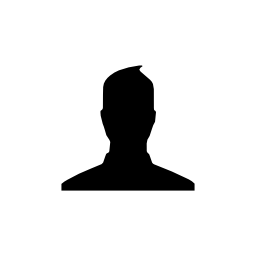
\includegraphics[scale=0.2]{images/fbuser.png}}
                (0,0) node [block] (fb) {
\includegraphics[scale=0.12]{images/fb_icon.png}}
                (5.5, 0) node [block] (friends) {
\includegraphics[scale=0.3]{images/fbfriends.png}}

                %Top part (PKG lists)
                (-3,4) node [block] (linkedin) {
\includegraphics[scale=0.1]{images/linkedin.png}}
                (-4,5) node [block] (fbpkg) {
\includegraphics[scale=0.06]{images/fb_icon.png}}
                (1.2,5) node [block] (gplus) {
\includegraphics[scale=0.08]{images/gplus.png}}
                (-2,5.2) node [block] (tumblr) {
\includegraphics[scale=0.1]{images/tumblr.png}}
                (2.8,4) node [block] (pin) {
\includegraphics[scale=0.05]{images/pinterest.png}}
                (4.2,5) node [block] (tor) {
\includegraphics[scale=0.1]{images/tor.png}}
                (-0.5,4) node [block] (twitter) {
\includegraphics[scale=0.05]{images/twitter.png}};

            \node[below=of fb] {\textbf{Facebook}};
            \node[below=of user] {\textbf{User}};
            \node[below=of friends] (frdcaption) {\textbf{Subset of Recipients}};
            \node[below=of frdcaption] {\textbf{s.t., $\mathcal{S}=\{\id{1},\id{2},\ldots,\id{\eta}\}$}};


            \begin{scope}[every path/.style=line]
                \path (user.east) -- (fb.west);               
            \end{scope}   

            % Legend
            \path (-2.8,0.35) node [leg] {Publish: $C\leftarrow$ Encrypt(\msg,$\mathcal{S}$)};
            \path (2.7,0.35) node [leg] {Retrieve $C$};
            \node[right=of friends] {Decrypt($C$)};
                
            \begin{scope}[every path/.style=line2]
                \path (fb) -- (friends);
                \path[dashed] (friends.north) -- (tor.south);
                \path[dashed] (5.1,1) -- (3.1,3.4);
                \path[dashed] (4.7,0.95) -- (0.5,3.5);
            \end{scope}
        \end{tikzpicture}
    }
    \end{center}
    \caption{Multiple $(n,t)$-PKG IBE for OSNs overview, for a message \msg\ published for the set $\mathcal{S}$ for $t=3$.}
    \label{fig:overview}
\end{figure}
% -----------------------------------------------------------------------------

% \begin{itemize}
%     \item Motivate the Multiple servers, e.g., assumptions that business model does not allow , and example open id. Also that requires at least t compromised PKGs to possible get the key -> point that this is hard
%     \item motivate new strategy that users can encrypt to other users even if the others don't run the system YET.
%     \item mention that efficiency for average users.
%     \item extension to scramble implementation, encryption is stored in servers and the link to the OSN
%     \item highlight that the key needs to be updated only once every month (for instance)
%     \item using VSS users can verify if the shares are valid ones and detect possible malicious PKGs and then announce
% \end{itemize}

\subsection{Contribution:} In this paper, we propose a novel practical solution that uses IBE with multiple untrusted PKGs atop of current OSNs. 
We highlight the fact that those multi-PKGs can be supported by several existing OSNs under the business competition assumption, and motivated by the possible attractive incentives towards more privacy concerned audience. 
Along with the multi-PKG IBE model we devise an IBE broadcast encryption protocol to support multiple recipients. Using a broadcast IBE-based mechanism we allow users to share content with multiple recipients, even if they are not using the system, and, thus, enforce confidentiality of the data while hiding the recipient set. Finally, we implemented our solution on top of the Scramble Firefox extension~\cite{BeatoScramble}, and show that only a small overhead is required.
 
\subsection{Roadmap:} The remainder of this paper is organized as follows. \secref{sec:background} gives a brief overview of the cryptographic background. Next, \secref{sec:model} presents the model followed by the description of the suggested solution in \secref{sec:solution}. \secref{sec:impl} describes the implementation details, while \secref{sec:relwork} reviews related work. Finally, \secref{sec:conc} summarizes and concludes the paper.

\section{Background}\label{sec:background}
In this section we briefly overview the cryptographic tools and building blocks used in this paper. For ease of explanation we omit the definitions of the underlying cryptographic primitives. This section 
can, however, be skipped with no loss of continuity.

\subsection{Identity Based Encryption}
The concept of Identity Based Encryption (IBE) was introduced by Shamir~\cite{DBLP:conf/crypto/Shamir84}, with the main idea of using any string as the public key. IBE requires no certificates as users can rely on publicly known identifiers such as an e-mail address or a telephone number, thus, reducing the complexity of establishing and managing a public key infrastructure. Boneh and Franklin propose the first practical IBE using bilinear pairings \cite{BonehFranklinIBE}, later extended by Gentry~\cite{GentryRandomOracles}. 

A generic IBE scheme is composed of four randomized algorithms:
\begin{description}
    \item[\texttt{IBE.Setup:}]~\\ On the input of a security parameter $\lambda$, outputs a master secret $s$ and the master public parameters $params$. 
    \item[\texttt{IBE.Extract:}]~\\ Takes the public parameters $params$, the master secret $s$, and an \id{} and returns the private key $d_{\id{}}$.
    \item[\texttt{IBE.Encrypt:}]~\\ Returns the encryption $C$ of the message \msg\ on the input of the $params$, the \id{}, and the arbitrary length message \msg. 
    \item[\texttt{IBE.Decrypt:}]~\\ Reconstruct \msg from $C$ by using the secret $d_{\id{}}$.
\end{description}

The \texttt{IBE.Setup} and \texttt{IBE.Extract} algorithms are executed by a trusted Private Key Generator (PKG) server, whereas \texttt{IBE.Encrypt} and \texttt{IBE.Decrypt} are performed by two players, e.g., Alice and Bob. Consequently, key escrow is performed implicitly in the classic IBE scheme as the PKG holds the master secret key.

\subsection{Anonymous Broadcast Encryption}
Broadcast encryption (BE) was introduced by Fiat and Naor~\cite{FiatBE}, as a public-key generalization to a multi user setting. A BE scheme allows a user to encrypt a message to a subset $\mathcal{S}$ of users, such that, only the users in the set $\mathcal{S}$ are able to decrypt the message. The computational overhead of the BE is generally bound to the ciphertext and the number of recipients. To overcome this issue, the set $\mathcal{S}$ of recipients is generally known. Barth et al.~\cite{BarthBonehWaters} and Libert et al.~\cite{LibertANOBE} extended the notion of BE and introduced the notion of Anonymous Broadcast Encryption (ANOBE) scheme, where the recipient set $\mathcal{S}$ remains private even to the members in the set. Fazio and Perera~\cite{FazioOutsiderANOBE} suggested the notion of outsider anonymous BE that represents a more relaxed notion of ANOBE.  

A generic BE and ANOBE scheme consists of four randomized algorithms:
\begin{description}
    \item[\texttt{BE.Setup:}]~\\ On the input of a security parameter $\lambda$, generates the public parameters $params$ of the system.
    \item[\texttt{BE.KeyGen:}]~\\ Returns the public and private key ($pk,sk$) for each user according to the $params$.
    \item[\texttt{BE.Encrypt:}] Takes the set $\mathcal{S}=\{pk_i \ldots pk_{|\mathcal{S}|}\}$ along with the secret message \msg\ and generates $C$.
    \item[\texttt{BE.Decrypt:}]~\\ Reconstructs \msg\ from $C$ using the private key $sk_i$ if the corresponding public key $pk_i \in \mathcal{S}$. Otherwise, return $\bot$.
\end{description}

Note that the $pk$ can be represented by the \id{} value from the IBE scheme. 


\subsection{Distributed Key Generation}
Distributed Key Generation (DKG) was introduced by Pedersen~\cite{Pedersen:1991:NIS:646756.705507} to allow a group of entities to collaboratively setup a secret sharing environment over a public channel.
Secret sharing was introduced by Shamir~\cite{Shamir1979} and consists of dividing a secret \K\ into $n$ shares among $n$ entities, such that, only a subset of size greater than or equal to a threshold $t$ can reconstruct \K, where $t \geq n$. In practice, a random secret \K\ is generated along with a polynomial $f(x)$ of degree $t-1$ such that $f(0)=\K$, where the shares $s_i$ are represented by different points on the polynomial. Any entity with $t$ or more shares can reconstruct $f(x)$ using Lagrange interpolation, and subsequently find $\K$. Further, Chor et al.~\cite{DBLP:conf/focs/ChorGMA85} suggested a Verifiable Secret Sharing (VSS) scheme to allow anyone to verify that the right shares are used. The scheme was extended by Feldman~\cite{Feldman:1987:PSN:1382440.1383000} and Pedersen~\cite{Pedersen:1991:NIS:646756.705507}. 

For multiple parties to jointly generate a secret sharing \K, all entities are required to participate in a DKG scheme. Each entity $i$ involved generates a different $\K_i$ and $f^i(x)$, and later on distributes and verifies the shares $s_{ij}$. Hence, a generic DKG does not require a trusted party, as the master secret is computed as the sum of all the polynomials and can only be retrieved by joining $t$ shares. A generic DKG protocol consists of two phases:

\begin{description}
    \item[\texttt{DKG.Setup:}]~\\ Every entity $i$ generates a random secret $\K_i$ and computes a polynomial of degree $t-1$. The entity $i$ Distributes a valid share $s_{ij}$ over all the other $j$ entities, along with the commitment to the share. Each entity $j$ verifies the shares and computes the new share $s_j = \sum_i s_{ij}$. The master secret is unknown by each party, and composed by the origin point on the sum of all polynomials $f^i(x)$.
    \item[\texttt{DKG.Reconstruct:}]~\\ Each entity $i$ broadcasts its share $s_i$, and with $t \leq n$ shares, one can reconstruct the master secret $s$.
\end{description}

The DKG protocol is secure assuming that no adversary is able to corrupt $t$ parties or more. 


\section{Model}\label{sec:model}
We consider that a user $u$ to be a member of an OSN, such as Facebook, Twitter or Google+. Such $u$ is connected with other users in the same OSN by a friendship relation with who shares information~\cite{boyd2008social}. Inherently, $u$ aims to interact and share information \msg\ with other users. Each user holds a public and private key pair which is given by an IBE identity server (composed of multiple PKG servers), such that the public key is represented by the \id{} of the user in the OSN. Note that each user can be registered into multiple OSNs and hold different public keys and \id{}s. We assume that the authentication between the user and the identity servers is done using a token similarly to open id, and performed under an authenticated channel, e.g., TLS.

% Don't we want users to be able to discuss on updates of common friends without the need for these users to be a connection on the OSN?

\paragraph{Threat Model:}
We consider an adversary to be any entity attempting to passively access the shared information \msg\ by monitoring the sharing channel but with no motivational incentive to tamper with the content. This can be any curious user in the OSN, the OSN provider or even a government agency~\cite{prism}. Such an adversary should not learn the content nor the identity of the members in the recipient set $\mathcal{S}$, otherwise we consider that the adversary breaks confidentiality and the outsider recipient anonymity of the protocol as defined in~\cite{FazioOutsiderANOBE}.
In addition, we assume that such an adversary cannot compromise more than $t$ identity servers.  Furthermore, we stress that such adversary cannot control the user computing environment. Also, it is hard to protect against a malicious recipient who copies or forwards shared content. In this case, we say that such recipient breaks the social contract. We stress that we offer no protection against traffic analysis or timing attacks. 


\paragraph{Goals:}
We aim to protect OSN users' privacy by ensuring confidentiality, data integrity and outsider recipient anonymity~\cite{FazioOutsiderANOBE}. In this way we allow users to enforce access control without having to rely on the privacy preferences offered by the OSN. At the same time, we aim at limited modifications to the OSN environment. In particular, we require as little  effort as possible and prior knowledge from users in order to achieve a user-friendly scheme as defined by Balsa et al.~\cite{article2400}. In contrast to previous solutions, users are allowed to be in the recipient set by default.


\section{Practical IBE for OSNs}\label{sec:solution}

In this section, we describe our system. The proposed solution is based on the IBE scheme from Boneh et al.~\cite{BonehFranklinIBE} and a relaxed version of the broadcast scheme from Libert et al.~\cite{LibertANOBE}. Further, the system relies on a DKG protocol as described by Pedersen~\cite{Pedersen:1991:NIS:646756.705507} to bootstrap multiple PKGs. In addition, we converted the schemes from using Type 1 (i.e., $\mathbb{G}_1 = \mathbb{G}_2$) to Type 3 (i.e., $\mathbb{G}_1 \neq \mathbb{G}_2$) pairings for efficiency~\cite{Galbraith:2008:PC:1450345.1450543} and because Type 1 pairings are no longer secure according Joux in~\cite{DBLP:journals/iacr/Joux13}.


\subsection{Basic Scheme}

Let $\lambda$ be the security parameter for a security level of $l$ bits, and $\mathcal{S}$ the set of desired recipients $u_i$ with corresponding \id{i}, such that $\mathcal{S} = \{u_1,..,u_\eta\}$ where $\eta=|\mathcal{S}|$. Let $\mathcal{G}$ be a generator that satisfies the Bilinear Diffie-Helman (BDH) assumption, and $e: \mathbb{G}_1 \times \mathbb{G}_2 \rightarrow \mathbb{G}_T$ the bilinear map such that $e \left( aP, bQ \right) = e \left( P, Q \right)^{ab}$ for $P \in \mathbb{G}_1, Q\in \mathbb{G}_2$ and $a,b \in \mathbb{Z}_q$ as in~\cite{BonehFranklinIBE} .
In addition, let $\{ C, T\} \leftarrow \mathtt{E}_k(M)$ be any secure authenticated symmetric encryption that takes as input the plaintext $M$ and generates ciphertext $C$ and authentication tag $T$ as output~\cite{rfc5288}. Similarly, $\{ M, T \} \leftarrow \mathtt{D}_k(C)$ be the valid authenticated decryption that takes ciphertext $C$ as input and computes the plaintext $M$ along with an authentication tag $T$. 
Our scheme for OSNs is composed by five randomized algorithms: \texttt{Setup}, \texttt{KeyGen}, \texttt{Publish}, and \texttt{Retrieve}.

\medskip

\begin{description}
    \item[\texttt{Setup($\lambda, t, n$)}:]~\\ Outputs the public $params$ of the system with respect to the security parameter $\lambda$, the number of PKGs $n$ and the threshold $t$.
    \begin{enumerate}
        \item On input of security parameter $\lambda$ generate a prime $q$, two groups $G_1, G_2$ of order $q$, and an admissible bilinear map $e: G_1 \times G_2 \rightarrow G_T$. Choose random generators $P \in G_1$ and $Q \in G_2$. 
    
        \item Choose cryptographic hash functions $H_1: \{ 0,1 \}^{*} \rightarrow G_1$, ${H_2: G_T \rightarrow \{ 0,1 \}^{l}}$ and $H_3: \{ 0, 1 \}^{l} \rightarrow \{ 0,1 \}^{l}$ such that, $H_1, H_2$ can be modelled as random oracles.
        
        \item Each PKG $j$ generates $n-1$ shares $\sigma_{jv}$ of a Pedersen VSS scheme by executing \texttt{DKG.Setup}, and redistributing the $n-1$ shares $\sigma_{jv}$ with the other $v$ PKGs.

        \item Each PKG $j$ publishes $P_{pub}^{(j)} = s_j P$, s.t., $s_j=\sum_{v=1}^n \sigma_{jv}$.
    \end{enumerate}
    
    The master secret key $msk = \sum_{j \in \Lambda} b_j s_j$ for $b_j = \prod_{z \in \Lambda} \frac{z}{z-j}$ cannot be retrieved unless $\Lambda$ is a subset of size $t$ different PKG servers. The following parameters are published publicly:
    \begin{equation*}
    \begin{split}
    params = \{ q, G_1, G_2, e, P, Q, H_1, H_2, H_3, \\ t, n, P_{pub}^{(0)}, \ldots, P_{pub}^{(n)} \}
    \end{split}
    \end{equation*}
    
    \bigskip

    \item[\texttt{KeyGen(\{PKG$_0,\ldots,$PKG$_t\}, \id{i}$)}:]~\\ On input of a user $\id{i}$ the subset $\Lambda$ of size $t$ of PKG servers, generates a valid private key for \id{i}. 
    
    \begin{enumerate}
        \item User with identifier \id{i}, authenticates to $\Lambda$ or all PKGs and sends \id{i}.
        \item Each PKG computes $Q_{\id{i}} = H_1 \left( \id{i} \right)$, and $Q_{priv,\id{i}}^{(j)} = s_j Q_{\id{i}}$, where $s_j$ is the secret share from PKG $j$.
        \item The user $\id{i}$ computes the shared public parameter $P$ using the Lagrange coefficients $b_j$ as follows:
        \begin{equation*}
         P = \sum_{j \in \Lambda} b_j P_{pub}^{\left( j \right)} \quad \textrm{for} \quad b_j = \prod_{z \in \Lambda} \frac{z}{z-j}
        \end{equation*}
        \item All PKGs in $\Lambda$ return $Q_{priv,\id{i}}^{(j)}$ to the corresponding user $\id{i}$ over a secure channel.
        \item Each user verifies for each $Q_{priv,\id{i}}^{(j)}$ value whether, 
        \begin{equation*}
            e \left( Q_{priv , \id{i} }^{(j)}, P \right ) \stackrel{?}{=} e \left( Q_{\id{i}}, P_{pub}^{(j)} \right)
        \end{equation*}
        
        %If the check fails, report that PKG as malicious and request another PKG. 
        Next, $\id{i}$ calculates the private key $s_{\id{i}}$ using the Lagrange coefficients $b_j$ as follows: 
        \begin{equation*}
            s_{\id{i}} = \sum\limits_{j\in\Lambda} b_j Q_{priv,\id{i}}^{(j)} \quad \textrm{for} \quad b_j = \prod_{z\in \Lambda} \frac{z}{z-j}
        \end{equation*}
        \end{enumerate}
        In this way, no user or PKG learns the master key $msk$ of the system. This algorithm combines \texttt{DKG.Reconstruct}, \texttt{IBE.Extract} and \texttt{BE.KeyGen} algorithms.
        \bigskip
\item[\texttt{Publish($params, \mathcal{S}, m$)}:]~\\ Takes the message $m$, the subset $\mathcal{S}$ of size $\eta$ and the public parameters $params$, output a broadcast message $\mathcal{B}$.

    \begin{enumerate}
        \item Generate a random symmetric session key $k \leftarrow \{ 0,1 \}^{l}$.
        \item Choose a random value $\rho \in \{ 0,1 \}^{l}$ and compute $r$ as a hash of concatenated values $r = H_3 \left( \{ \rho \parallel k \} \right)$
        \item For each recipient $\id{i} \in \mathcal{S}$, compute the ciphertext, running the \texttt{IBE.Encrypt} algorithm, as follows.
            \begin{equation*}
            \begin{array}{ll}
                w_i = & \rho \oplus H_2 \left( g_{\id{i}}^r \right)  \\ & \textrm{where} \; \; \; g_{\id{i}} = e \left( Q_{\id{i}}, P_{pub} \right) \in G_T
            \end{array}
            \end{equation*}
        \item Let $w$ be a randomised concatenation, then the authenticated data $\mathcal{A}$ is computed as                                  
        \begin{equation*}
                \begin{array}{lcl}
                    \mathcal{A} & = & \{ \eta \parallel rP \parallel k \oplus H_3 \left( \rho \right) \parallel w_1  \parallel \ldots \parallel w_\eta \} \\
                    & = & \{ \eta \parallel U \parallel v \parallel w \} \\
                    & & \textrm{for}\; \; \; w = \{ w_1 \parallel w_2 \parallel \ldots \parallel w_\eta \}
                \end{array} 
            \end{equation*}
            
        And $\mathcal{M}$ a concatenation of the intended recipient set $\mathcal{S}$ and the plaintext message $m$, such that $\mathcal{M} = \{ m \parallel \mathcal{S} \}$. (\texttt{BE.Encrypt})
    
        \item Apply authenticated symmetric encryption
        \begin{equation*}
            \left< c, t \right> \leftarrow \mathtt{E}_k(\mathcal{M},\mathcal{A})
        \end{equation*}
        \item The following message is then published in the OSN
        \begin{equation*}
            \mathcal{B} = \{ \mathcal{A} \parallel t \parallel c \}
        \end{equation*}
    \end{enumerate}
    
    \bigskip
    
    \item[\texttt{Retrieve($params, s_{\id{i}}, \mathcal{B}$)}:]~\\ on input of the broadcast message $\mathcal{B}$ and the private key $s_{\id{i}}$ of user $\id{i}$, reconstruct the plaintext message $m$. This algorithm comprises the \texttt{\{IBE,BE\}.Decrypt} algorithms. For each $i \in \{  \}$ \\

    \begin{enumerate}
        \item Compute $w_i \oplus H_2 \left( e \left( s_{\id{i}}, U \right) \right) = \rho$ for $s_{\id{i}}$, and $v \oplus H_3 \{ \rho \} = k$ 
        \item Set $r = H_3 \left( \rho, k \right)$. Verify $U \stackrel{?}{=} rP$. If the check fails, try next $W_i$ and return to 1.
        \item Retrieve $\left< \mathcal{M}, t' \right> \leftarrow \mathtt{D}_k(c, \mathcal{A})$
        \item Verify whether $t' \stackrel{?}{=} t \in \mathcal{B} $, and return $m$. Otherwise return $\bot$. 
    \end{enumerate}
\end{description}



\subsection{Evaluation}

Our solution achieves confidentiality, integrity and outsider recipient anonymity as in~\cite{BarthBonehWaters,BonehFranklinIBE,FazioOutsiderANOBE},because the session key can only be obtain if the recipient holds the corresponding secret key $d_{\id{i}}$ and as a consequence of the authenticated encryption. Our solution can also be used in any OSN that assigns unique public \id{}s, such as usernames. As the public keys are represented as strings  users are not required to upload keys to an additional third party server. The DKG approach solves the key escrow issues that come with IBE solutions.

In terms of efficiency, users are required to decrypt $W_i$ on average $O\left( n/2 \right)$ before obtaining the symmetric key $k$. Both Barth et al.~\cite{BarthBonehWaters} and Libert et al.~\cite{LibertANOBE} propose using a tag based system to hint users where their symmetric key can be found. However, as a design choice we deliberately decided to not implement such property in the scheme as it introduces a linear dependency from extra public parameters to the users, i.e., there are extra public parameters that need to be shared and verified. Using IBE allows any user in the OSN to be part of the recipient set $\mathcal{S}$ before registering in the system. In addition, users can reuse (a hash of) the same symmetric key $k$ during the comments and discussion phase. If the users opt not to reuse $k$ they can still encrypt a fresh session key to all recipients in $\mathcal{S}$ using $k$.

In contrast to classic public key infrastructure, if a public key in IBE is revoked, the user would no longer be able to use that identifier for encryption, e.g., Facebook \id{}. Therefore, to support revocation an expiration date is concatenated to the identifier~\cite{BonehFranklinIBE}. 

For the multi-PKG setting, a user is able to detect malicious behavior from the public commitments of the Pedersen VSS~\cite{Pedersen:1991:NIS:646756.705507}. It is also required that at least $t$ from $n$ PKGs do not get compromised, thus, the higher threshold $t$ the higher the level of security. In case the OSN providers would maintain the PKG infrastructure, one could rely on the assumption that direct business competitors do not collude nor get legally coerced. Furthermore, the authentication and identity verification to the different servers can be done via, for instance, an open id token. This token is generated as a proof of identity by any of the OSN providers.


\section{Practicalities}\label{sec:impl}
To demonstrate the viability of our solution, we implemented a proof-of-concept prototype of the distributed identity based broadcast encryption scheme for OSNs.\footnote{Source of our implementations is available upon request.} In this section, we discuss the implementation details and the performance results of the cryptographic blocks.

\paragraph{Implementation:}
For the client component we modified the cryptographic library from Scramble~\cite{BeatoScramble} as it is an available open source privacy preserving project. In addition, Scramble is implemented as a Firefox Extension compatible with Firefox 14+, but as it is written in simple Javascript it could easily be ported to other browsers, e.g., Chrome. 
We implemented the multiple PKG servers in PHP.
The bilinear pairing and cryptographic blocks for the PKG and the client component are implemented using the multi-precision {MIRACL} library~\cite{scott2003miracl}. To overcome the limitation of accessing binary code from a browser extension implementation, a local client-server socket implementation was used to perform the cryptographic requests to the developed scheme using the {MIRACL} library.
For the DKG protocol we implemented a primitive version of Pedersen's DKG protocol~\cite{art:Pedersen91a} to generate the collective master secret key for the $(n,t)-$PKG servers. Adaption to the asynchronous setting could be done with the available implementation from Kate and Goldberg~\cite{DBLP:conf/icdcs/KateG09,dkg-software}. AES-GCM~\cite{rfc5288} was used for the authenticated encryption. For the public key the Facebook username was used, i.e., $\id{}=facebook.com/user.name$. 


\paragraph{Performance:} 
Experiments were conducted on a Intel Core 2.4 GHz i5 processor with 8 Gb of 1600 MHz DDR3L onboard memory. Table~\ref{table:BE_exec_times} illustrates the 
execution times for the scheme proposed in \secref{sec:solution} for $\lambda=256$ bits. Each recipient has to decrypt $W_i$ an average of $n/2$ times to retrieve the secret and subsequently decrypt the secret message \msg. Note that efficiency comes at the cost of the recipient anonymity $\mathcal{S}$, as to hide $\mathcal{S}$ it is required to produce more \texttt{IBE.Encrypt} calls.

\begin{table}
  \centering
  \begin{tabular}{@{}rrr@{}} \toprule
    \multicolumn{3}{r}{Execution Time (ms)} \\ \cmidrule(r){2-3}
    Number of Recipients & \texttt{Publish} & \texttt{Retrieve} \\ \midrule
    %%%%%%%%%%%%%%%%%%%%%
    % CCA Secure scheme %
    %%%%%%%%%%%%%%%%%%%%%
    1 & 284.5 & 275.4  \\
    % 5 & 1278.750 \ms & 357.302 \ms \\
    10 & 2564.5  & 460.9  \\
    15 & 3799.6  & 560.6  \\
    % 20 & 5029.470 \ms & 657.030 \ms \\
    % 25 & 6258.510 \ms & 761.765 \ms \\
    50 & 12300.5  & 1237.8  \\
    100 & 25867.7  & 2260.2  \\  \bottomrule
    & & \\
  \end{tabular}
  \caption{Performance of the \texttt{Publish} and \texttt{Retrieve} stages in function of the number of intended recipients.}
  \label{table:BE_exec_times}
\end{table}

We also analyzed the execution times of the IBE scheme, as it represents the most costly part of the scheme. Furthermore, our solution uses the random oracle assumption; we show in \tabref{table:exec_times} that there is a significant computational difference between a similar scheme in the standard model, i.e., Gentry~\cite{GentryRandomOracles}.
Nevertheless, we believe that our solution presents a tolerable cost to average users with 100 friends and a usual group size of 15~\cite{DBLP:journals/corr/abs-1111-4503}. 

\begin{table}
  \centering
  \begin{tabular}{@{}lrr@{}} \toprule
    \multicolumn{3}{r}{Execution Time (ms)} \\ \cmidrule(r){2-3}
    IBE Stage & Boneh and Franklin & Gentry \\ \midrule
    \texttt{IBE.Setup} & 368.10  &  424.49  \\
  \texttt{IBE.Extract} & 13.84  & 37.46  \\
  \texttt{IBE.Encrypt} & 271.90  & 1136.65  \\
  \texttt{IBE.Decrypt} & 252.82  & 911.32 \\ \bottomrule
    & & \\
  \end{tabular}
  \caption{Comparison of execution time for different IBE schemes.}
  \label{table:BE_exec_times}
\end{table}

\section{Related Work}\label{sec:relwork}
The increased popularity of Online Social Networks (OSNs) and the amount of disseminated information prompted several privacy concerns. 
Guha et al.~\cite{Guha:2008} proposed NOYB a solution that replaces the personal details of users by fake information. Later, FaceCloak~\cite{Luo:2009} and Scramble~\cite{BeatoScramble} make use of cryptographic mechanisms to enforce privacy to the published information. Further, Persona suggest an attribute based encryption scheme for social networks. However, all the aforementioned solutions suffer from a complex key management infrastructure. 


Other solutions take a more drastic approach by proposing novel, privacy-friendly architectures meant to replace existing platforms~\cite{DBLP:conf/sp/CristofaroSTW12,NYT2010.Diaspora,DBLP:conf/wowmom/CutilloMO11}. Besides the privacy protection offered, these solutions face a reduced user wilingness to adopt to a new platform.

Recently, Jung et al.~\cite{jung} proposed a key management scheme based on dynamical IBE for decentralized OSNs. Their scheme, however, presents several problems. Foremost contains a single point of failure as a trusted party should generate the secret keys for a given \id{}. This proposal still requires an additional public key that needs to be certified and shared among other users for the broadcasting, thus, not solving the key management issue.

In general all previous schemes require public parameters that should be shared and verified by users. In addition, by using an Identity-based scheme we allow users to motivate their friends to use the solution, as registered users can already encrypt messages to unregistered friends.



\section{Conclusion}\label{sec:conc}

Identity Based Encryption (IBE) solutions provide desirable properties to construct mechanisms to deliver privacy in OSNs. The minimal
additional architectural support and the increased ease of key management represent a major motivation to implement IBE in OSNs. We show that using secret sharing and multi-PKGs there is no need to have a single trusted party, assuming that at least $t-1$ of the PKGs are compromised. 
Furthermore, the multiple PKG infrastructure can be maintained by several OSN providers, motivated by the attractive OSN privacy-friendly label, incentives towards more privacy concerned users, and considering the business model. 
Hence, users are provided with the option to use multiple identities, that they can use interchangeably among OSNs, e.g., use Twitter \id{} as a public key in Facebook. 
In contrast to previous solutions, it is possible to share content with users not holding private keys to their identity as the valid public key is directly represented by their \id{} in the OSN. This forces curious users to register if they wish to view the protected content shared with them.
Lastly, we have extended Scramble and demonstrated that such extension presents a tolerable overhead to end-users. 
There are some important open challenges that call for further research. We endeavor to obtain a full open source project that supports different browsers. Items like a more detailed security discussion and efficiency improvement are also important and required. In addition, for the authentication and proof of identity we foresee several open challenges to increase user privacy and security, as well as adoption of the scheme.


% An example of a floating figure using the graphicx package.
% Note that \label must occur AFTER (or within) \caption.
% For figures, \caption should occur after the \includegraphics.
% Note that IEEEtran v1.7 and later has special internal code that
% is designed to preserve the operation of \label within \caption
% even when the captionsoff option is in effect. However, because
% of issues like this, it may be the safest practice to put all your
% \label just after \caption rather than within \caption{}.
%
% Reminder: the "draftcls" or "draftclsnofoot", not "draft", class
% option should be used if it is desired that the figures are to be
% displayed while in draft mode.
%
%\begin{figure}[!t]
%\centering
%\includegraphics[width=2.5in]{myfigure}
% where an .eps filename suffix will be assumed under latex, 
% and a .pdf suffix will be assumed for pdflatex; or what has been declared
% via \DeclareGraphicsExtensions.
%\caption{Simulation Results.}
%\label{fig_sim}
%\end{figure}

% Note that IEEE typically puts floats only at the top, even when this
% results in a large percentage of a column being occupied by floats.


% An example of a double column floating figure using two subfigures.
% (The subfig.sty package must be loaded for this to work.)
% The subfigure \label commands are set within each subfloat command,
% and the \label for the overall figure must come after \caption.
% \hfil is used as a separator to get equal spacing.
% Watch out that the combined width of all the subfigures on a 
% line do not exceed the text width or a line break will occur.
%
%\begin{figure*}[!t]
%\centering
%\subfloat[Case I]{\includegraphics[width=2.5in]{box}%
%\label{fig_first_case}}
%\hfil
%\subfloat[Case II]{\includegraphics[width=2.5in]{box}%
%\label{fig_second_case}}
%\caption{Simulation results.}
%\label{fig_sim}
%\end{figure*}
%
% Note that often IEEE papers with subfigures do not employ subfigure
% captions (using the optional argument to \subfloat[]), but instead will
% reference/describe all of them (a), (b), etc., within the main caption.


% An example of a floating table. Note that, for IEEE style tables, the 
% \caption command should come BEFORE the table. Table text will default to
% \footnotesize as IEEE normally uses this smaller font for tables.
% The \label must come after \caption as always.
%
%\begin{table}[!t]
%% increase table row spacing, adjust to taste
%\renewcommand{\arraystretch}{1.3}
% if using array.sty, it might be a good idea to tweak the value of
% \extrarowheight as needed to properly center the text within the cells
%\caption{An Example of a Table}
%\label{table_example}
%\centering
%% Some packages, such as MDW tools, offer better commands for making tables
%% than the plain LaTeX2e tabular which is used here.
%\begin{tabular}{|c||c|}
%\hline
%One & Two\\
%\hline
%Three & Four\\
%\hline
%\end{tabular}
%\end{table}


% Note that IEEE does not put floats in the very first column - or typically
% anywhere on the first page for that matter. Also, in-text middle ("here")
% positioning is not used. Most IEEE journals use top floats exclusively.
% Note that, LaTeX2e, unlike IEEE journals, places footnotes above bottom
% floats. This can be corrected via the \fnbelowfloat command of the
% stfloats package.



% if have a single appendix:
%\appendix[Proof of the Zonklar Equations]
% or
%\appendix  % for no appendix heading
% do not use \section anymore after \appendix, only \section*
% is possibly needed

% use appendices with more than one appendix
% then use \section to start each appendix
% you must declare a \section before using any
% \subsection or using \label (\appendices by itself
% starts a section numbered zero.)
%


%\appendices
%\section{Proof of the First Zonklar Equation}
%Appendix one text goes here.

% you can choose not to have a title for an appendix
% if you want by leaving the argument blank
%\section{}
%Appendix two text goes here.


% use section* for acknowledgement
\section*{Acknowledgment}

This paper is the result of a one-year master’s thesis.
Therefore I would like to thank my promotors prof. dr. ir.
Bart Preneel and prof. dr. ir. Vincent Rijmen and the KU
Leuven to make this research possible. I would also like to
thank my daily supervisor Filipe Beato for helping me
with the reviewing, writing and implementation.

% Can use something like this to put references on a page
% by themselves when using endfloat and the captionsoff option.
\ifCLASSOPTIONcaptionsoff
  \newpage
\fi



% trigger a \newpage just before the given reference
% number - used to balance the columns on the last page
% adjust value as needed - may need to be readjusted if
% the document is modified later
%\IEEEtriggeratref{8}
% The "triggered" command can be changed if desired:
%\IEEEtriggercmd{\enlargethispage{-5in}}

% references section

% can use a bibliography generated by BibTeX as a .bbl file
% BibTeX documentation can be easily obtained at:
% http://www.ctan.org/tex-archive/biblio/bibtex/contrib/doc/
% The IEEEtran BibTeX style support page is at:
% http://www.michaelshell.org/tex/ieeetran/bibtex/
%\bibliographystyle{IEEEtran}
% argument is your BibTeX string definitions and bibliography database(s)
%\bibliography{IEEEabrv,../bib/paper}
%
% <OR> manually copy in the resultant .bbl file
% set second argument of \begin to the number of references
% (used to reserve space for the reference number labels box)
\bibliographystyle{IEEEtran}
\bibliography{references}

% biography section
% 
% If you have an EPS/PDF photo (graphicx package needed) extra braces are
% needed around the contents of the optional argument to biography to prevent
% the LaTeX parser from getting confused when it sees the complicated
% \includegraphics command within an optional argument. (You could create
% your own custom macro containing the \includegraphics command to make things
% simpler here.)

% or if you just want to reserve a space for a photo:

%\begin{IEEEbiography}{Stijn Meul}
%Biography text here.
%\end{IEEEbiography}

% if you will not have a photo at all:
%\begin{IEEEbiographynophoto}{John Doe}
%Biography text here.
%\end{IEEEbiographynophoto}

% insert where needed to balance the two columns on the last page with
% biographies
%\newpage

%\begin{IEEEbiographynophoto}{Jane Doe}
%Biography text here.
%\end{IEEEbiographynophoto}

% You can push biographies down or up by placing
% a \vfill before or after them. The appropriate
% use of \vfill depends on what kind of text is
% on the last page and whether or not the columns
% are being equalized.

%\vfill

% Can be used to pull up biographies so that the bottom of the last one
% is flush with the other column.
%\enlargethispage{-5in}



% that's all folks
\end{document}


